\section{BRUNET-DERRIDA CONJECTURES}

\subsection{Introduction to Branching-Selection Systems}
In this essay we will study Branching Random Walks with selection ($N$-BRWs), which the reader can think of as a cloud of particles on $\R$ indexed by discrete time. Loosely speaking these `branching-selection' systems evolve according to two mechanisms: 
\begin{enumerate}[1]
\item \textbf{branching} Each particle gives birth to offspring whose position is scattered on the real line. 
\item \vspace{-2mm}\textbf{selection} Out of all children, the rightmost $N$ are selected to form the next generation.
\end{enumerate}
Regular Branching Random Walks without selection (BRWs) correspond to the case $N = \infty$. For the models that we care about the branching step happens independently for each particle in the population. Moreover, each particle's offspring is distributed according to the same point process on $\R$ translated by the position of their parent. Of course one could also consider continuous time branching(-selection) systems, for example Branching Brownian Motion (BBM) which is one of the first and most natural such models to be studied. In standard/dyadic BBM the particles follow independent Brownian motions while branching independently at exponential rate $1$. At the time of branching the particle in question is replaced by two particles at the same position, who continue independently on their Brownian path. To this description it is then straightforward to add the selection step, which results in the $N$-BBM model. \\

\begin{figure}[!h]
\centering
\begin{minipage}{0.45\textwidth}
  \centering
  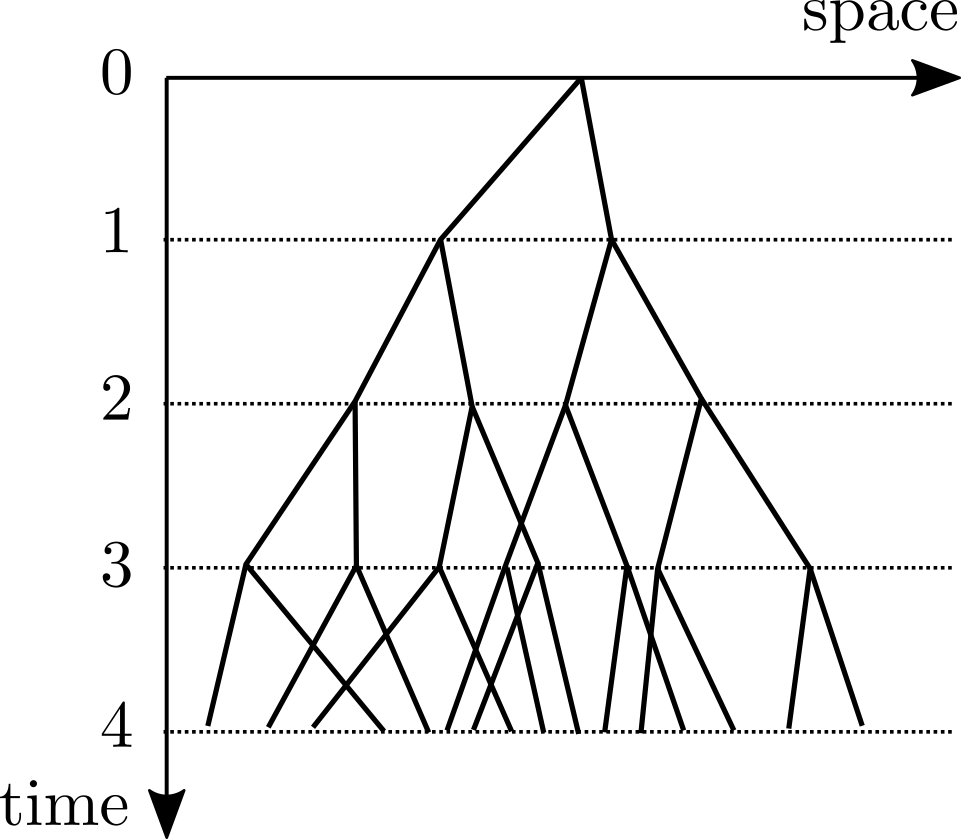
\includegraphics{graphics/binary_BRW}
  \caption{Sketch of a binary BRW. }
  \label{fig:binary_BRW}
\end{minipage}\hfill%
\begin{minipage}{0.45\textwidth}
  \centering
  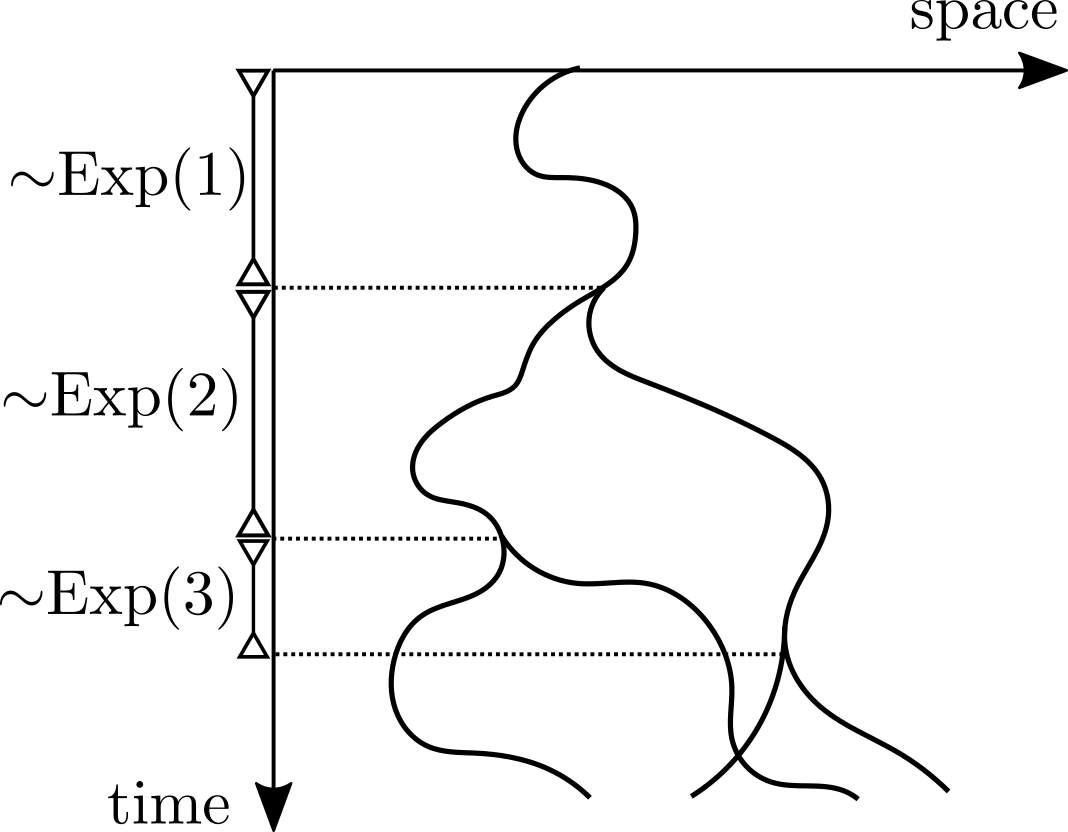
\includegraphics{graphics/binary_BBM}
  \caption{Sketch of a standard BBM. }
  \label{fig:binary_BBM}
\end{minipage}
\end{figure}

\begin{remark}[Related models]BRWs without selection and BBM have been studied extensively in the past. The book \cite{shi2015branching} gives a good overview of the results and methods employed in the study of BRWs, while Professor Berestycki's lecture notes\footnote{Said lecture notes can be found at \url{www.stats.ox.ac.uk/~berestyc/Articles/EBP18_v2.pdf}} give a good introduction to BBM. The introduction of selection makes the models significantly more difficult to study. However, many related models have been introduced. One such model is the BRW/BBM killed under a linear boundary. The idea is that instead of selecting the $N$ rightmost particles, the next generation is formed by the children whose position is greater than $v \times g$; where $v$ is some fixed velocity and $g$ is the current generation. Questions such as when the system survives, what speed the front propagates with and what the genealogical tree looks like are natural and have been studied for example in \cite{gantert2008asymptotics, harris2007survival, berestycki2013genealogy}. The notion of an $L$-BRW was introduced in \cite{brunet2006phenomenological} where only particles within distance $L$ to the rightmost particle survive. In \cite{cortines2016n} the authors studied a model in which exactly $N$ particles are selected, but in a random manner depending on the position of the particles. What we have listed here is just a fraction of the work on problems like these, however we hope it shows the reader the general level of interest of the community in this subject. 
\end{remark}








\subsection{Traveling waves and the FKPP-equation}\label{subsec:FKPP}
This section relies mainly on \cite{FKPP_origin} and partly on \cite[Section 2]{brunet2015exactly} to give an introduction to the FKPP-equation and its traveling wave solutions. Let $u:[0, \infty) \times \R \to [0,1]$ be sufficiently differentiable. The general form of the FKPP-equation as presented in \cite{FKPP_origin} is 
\begin{equation}\label{eqn:FKPP}
\frac{\partial}{\partial t} u(t, x) = \kappa \frac{\partial^2}{\partial x^2} u(t, x) + F(u)
\end{equation}
with $\kappa > 0$ and forcing term $F$ that satisfies 
\begin{align}\label{eqn:fkpp_assumption}
F(0) &= F(1) = 0 \\
F(u) &> 0, \,\,\forall\,u \in (0,1) \\
F'(0) &> 0 \text{ and } F'(u) < F'(0),\,\,\forall\,u\in(0, 1]. 
\end{align} 
Fisher \cite{fisher1937wave} was the first to study a special case of (\ref{eqn:FKPP}): he used (\ref{eqn:FKPP}) with $F(u) = u (1 - u)$ to describe the spread of a favorable gene over time in a population along one dimension where the function $u$ denoted the fraction of individuals posessing the gene at position $x$ at time $t$. It turns out that (\ref{eqn:FKPP}) is intimately related to problems of front propagation in many problems of physics, chemistry and biology. Kolmogorov, Petrovskii and Piskunov \cite{FKPP_origin} were the first to study the equation analytically and prove properties of the traveling wave solutions of the FKPP-equation. A function $w_v \in C^2$ is called a traveling wave solution if there exists $v \in \R$ such that $(t,x) \mapsto w(x + v t)$ solves the equation. The name `traveling wave' is descriptive: the solution $w_v(x + vt)$ to (\ref{eqn:FKPP}) is just a fixed shape $w_v:\R \to \R$ that travels to the left at speed $v$. Remarkably, the FKPP-equation is one of the simplest equations that admits traveling wave solutions. \\

\begin{figure}[!h]
\centering
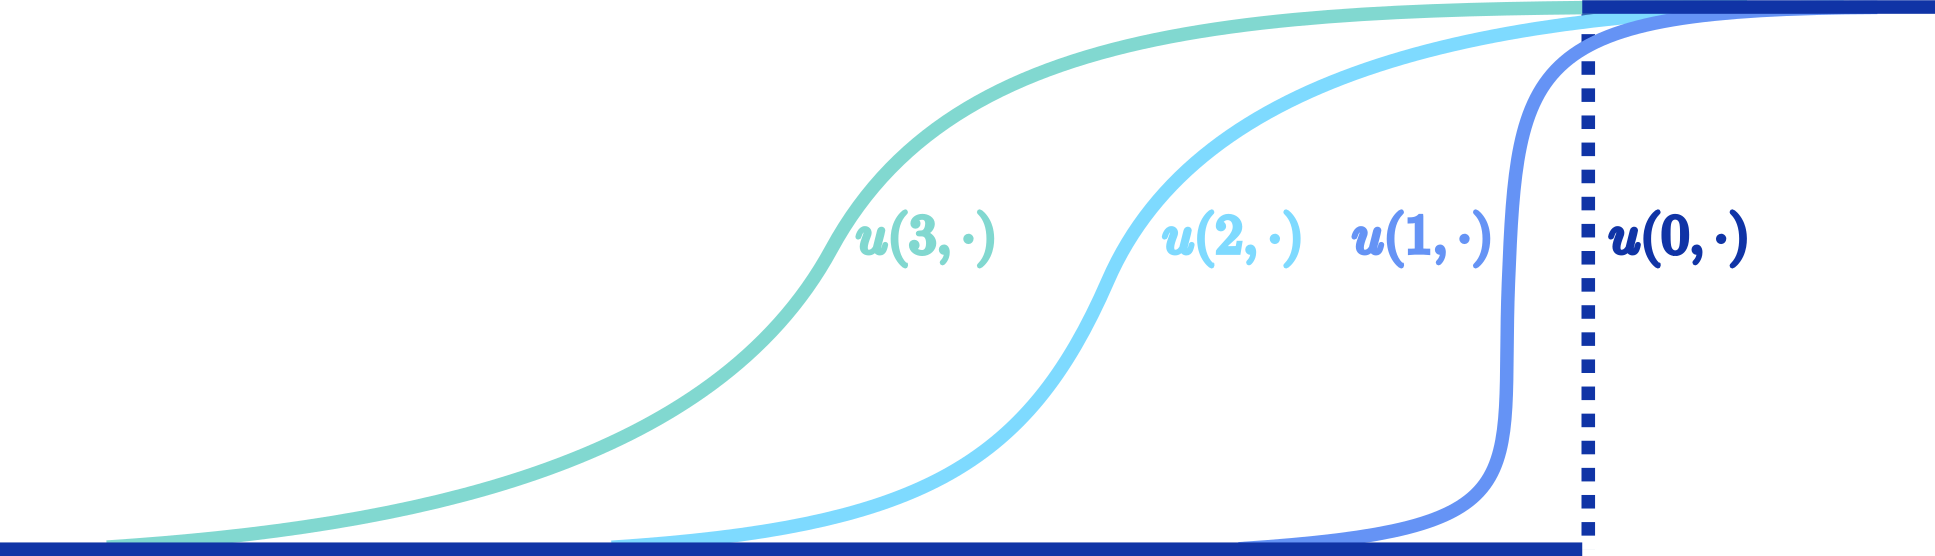
\includegraphics{graphics/waves_nonreflected}
\caption{A typical solution to the FKPP equation with initial data $\Ind_{\{ x > 0\}}$ (inspired by \cite{FKPP_origin}). }
\label{fig:waves}
\end{figure}


Suppose that we're interested in the case where the initial data is given by $u(0, x) \defeq \Ind_{\{ x > 0\}}$. A sketch of a typical solution can be found in Figure \ref{fig:waves}. We see that as $t$ grows, the shape seems to converge, while also moving to the left. The natural question to ask is then: what shape does it converge to, and what is limiting rate at which it propagates to the left. Instead of answering this straight away, let us look for a traveling wave solution $w_v$ to the FKPP equation which satisfies $w_v(-\infty) = 0$ and $w_v(\infty) = 1$. Substituting into (\ref{eqn:FKPP}) we see that $w_v$ must satisfy
\begin{equation}\label{eqn:wave_ODE}
v \frac{d}{dx}w_v(x) = \kappa \frac{d^2}{dx^2} w_v (x) + F(w_v). 
\end{equation}
With heuristic arguments following \cite{brunet2015exactly} (which can be made rigorous), we can deduce the possible values of $v$: for small values of $w_v(x)$ i.e. for large negative values of $x$ we can linearise (\ref{eqn:wave_ODE}) to get
\begin{equation}\nonumber
v \frac{d}{dx}w_v(x) = \kappa \frac{d^2}{dx^2}w_v(x) + F'(0) w_v. 
\end{equation}
It is easy to see that the above has a solution whose tail stays inside $[0,1]$ if and only if $v \geq 2 \sqrt{\kappa F'(0)}$. Further, the left tail of $w_v$ behaves like $e^{\gamma x}$ as $x \to -\infty$ where $\gamma$ is the smaller root of $v = \gamma \kappa + F'(0) / \gamma$. The smallest speed which admits a traveling wave solution, sometimes called the critical velocity, is denoted $v_c = 2 \sqrt{\kappa F'(0)}$ and the corresponding value of $\gamma$ by $\gamma_c = v_c / (2 \kappa)$. \\

Back to the problem of finding the limiting shape in Figure \ref{fig:waves}: we want to find conditions under which the solution `selects a speed' and what that speed is. More precisely, find conditions on $u(0, x)$ under which there exists $m : [0, \infty) \to [0, \infty)$ and $v \in \R$ such that
\begin{equation}\nonumber
u(t, x + m(t)) \to w_v \qquad\text{and}\qquad \frac{m(t)}{t} \to v
\end{equation} 
as $t \to \infty$, preferably uniformly in $x \in \R$. In the particular case when $u(0, x) = \Ind_{\{ x > 0\}}$ it turns out that 
\begin{equation}\nonumber
m(t) = v_c\,t - \frac{3}{2 \gamma_c} \log t + const. 
\end{equation}
works and the limit shape is $w_{v_c}$, as shown by Bramson \cite{bramson1978maximal}. The above in fact holds for more general initial conditions, in particular for ones with support bounded from below. \\

As mentioned before, the FKPP-equation has ties to many physical problems of interest. Branching Brownian motion is a well-studied probabilistic model that have a very precise connection to the FKPP-equation, with Bramson's works such as \cite{bramson1983convergence,bramson1978maximal} being fundamental in this topic. Recall the informal description of standard Branching Brownian Motion from the previous section. For each time $t \geq 0$ let $u(t, \cdot)$ denote the distribution function of the right-most particle's position at time $t$. We now present a short and informal proof of the fact that $1 - u(t, - x)$ satisfies the FKPP-equation with $F(u) = u(1 - u)$ and $\kappa = 1/2$, based on Professor Berestycki's lecture notes. Indeed, let $M(t)$ denote the position of the right-most particle at time $t$ so that $u(t, x) = \Pr{M(t) \leq x}$. For $dt > 0$ consider the right-most particle over the time interval $[t, t+dt]$:
\begin{itemize}
\item \vspace{-2mm}With probability $1 - dt + o(dt)$ it does not branch
\item \vspace{-2mm}With probability $dt + o(dt)$ it branches exactly once
\item \vspace{-2mm}With probability $o(dt)$ it branches more than once
\end{itemize}	
By the law of total probability and ignoring terms of order $o(dt)$ we find that 
\begin{align}
\Pr{M(t + dt) < x} &= (1 - dt)\, \Pr{M(t) \leq x - B_{dt}} + dt\, \Pr{M(t) \leq x}^2 + o(dt)\nonumber \\
				   &= \Ex{u(t, x - B_{dt})} + dt\, (u(t,x)^2 - u(t,x)) + o(dt). \label{eqn:fkpp-decomp} 
\end{align}
where $(B_t)_{t \geq 0}$ is an independent standard Brownian motion. Let $f(z) = u(t, z)$ so that $\Ex{u(t, x - B_{dt})} = \E_x f(B_{dt})$. Applying the Kolmogorov's backwards equation to $f$ (assuming $u(t, \cdot)$ is twice differentiable), we have 
\begin{equation}\nonumber
\lim\limits_{dt \downarrow 0} \frac{\Ex{u(t, x - B_{dt})} - u(t, x)}{dt} = \frac{1}{2} \frac{\partial^2}{\partial x^2} u(t, x). 
\end{equation}
Combining with (\ref{eqn:fkpp-decomp}) we get 
\begin{equation}\label{eqn:shitty_FKPP}
\frac{\partial}{\partial t} u(t, x) = \frac{1}{2} \frac{\partial^2}{\partial x^2} u(t, x) + u(t, x)(u(t, x) - 1)
\end{equation}
with initial condition
\begin{equation}\nonumber
u(0, x) = \Ind_{x \leq 0}. 
\end{equation}
After the transformation $\tilde{u}(t, x) = 1 - u(t, - x)$, (\ref{eqn:shitty_FKPP}) becomes the FKPP-equation with forcing term $F(\tilde{u}) = \tilde{u}(1 - \tilde{u})$ and initial condition $\tilde{u}(0, x) = \Ind_{\{ x > 0\}}$ so that $\tilde{u}$ selects the critical speed $v_c = \sqrt{2}$ so that the limit shape of $u$ propagates to the right at speed $\sqrt{2}$. \\








\subsection{Brunet-Derrida behaviour}
Assume for simplicity that $\kappa = 1$ in \ref{eqn:FKPP}. In their seminal paper \cite{brunet1997shift} Brunet and Derrida studied the FKPP-equation where the forcing term is multiplied by a cutoff $\Ind_{\{ u \geq \epsilon\}}$ and asked the question how the critical velocity $v_\epsilon$ behaves as $\epsilon \downarrow 0$. Using non-rigorous arguments they show that $v_\epsilon$ converges to $v_c$, the critical velocity of the problem without a cutoff. The speed at which this convergence occurs is found to be unusually slow:
\begin{equation}\label{eqn:brun_der_prediction}
v_\epsilon = v_c - \frac{\pi^2 \gamma_c^2 v''(\gamma_c)}{2 (\log \epsilon)^2} + o(1/(\log \epsilon)^2) 
\end{equation}
where $v(\gamma) = \gamma + F'(0)/\gamma$. They also introduce a discrete (in both space and time) front equation (and its cutoff version) which the authors then go on to relate to a probabilistic finite particle model whose limit is governed by said equation. The model, which appears in the study of directed polymers can be described as follows. Given $N \geq 1$ and $p \in (0,1)$, at any time $n \in \N$ there are $N$ particles alive at integer positions $x_1(n), ..., x_N(n)$, possibly multiple particles in the same position. For each $i \in [N]$ we choose $j^i_1, j^i_2 \in [N]$ uniformly at random and set $x_i(n+1) = x_{j^i_1}(n) + b^i_1 \land x_{j^i_2}(n) + b^i_2$ where $b^i_1, b^i_2$ are i.i.d. $\dBer{p}$. They define $h(n, m)$ to be the fraction of particles at time $n$ that fall above $m$ and show in a loose sense that $h(n,m)$ is governed by the discrete front equation in the limit $N \uparrow \infty$. The remarkable observation they make is that the asymptotic velocity $v_N$ of the stochastic model's rightmost particle converges to the critical velocity of the discrete front equation at rate $1/(\log N)^2$. Furthermore, based on the authors' large scale simulations, the constants seem to agree with their predictions of the critical speed of the discrete front equation with cutoff $\epsilon = 1/N$. \\

Consequently, the slow convergence rate $1 / (\log N)^2$ has become known as the 'Brunet-Derrida behaviour'. Along with it came several questions and conjectures
\begin{enumerate}[(i)]
\item \vspace{-2mm}Can we understand the relationship between branching(-selection) systems and the FKPP-equation (with cutoff)? 
\item \vspace{-2mm}What equations exhibit Brunet-Derrida behaviour? \label{item:eqns_brun_der_behav}
\item \vspace{-2mm}What branching-selection systems exhibit Brunet-Derrida behaviour? \label{item:systems_brun_der_behav}
\end{enumerate}{}
There has been progress towards answering (\ref{item:eqns_brun_der_behav}) in \cite{dumortier2007critical} where the authors prove the results of \cite{brunet1997shift} rigorously, in the case $f(u) = (u - g(u)) \times\,\phi(u)$ for a specified class of cutoffs $\phi$ including $u \mapsto \Ind_{\{ u \geq \epsilon\}}$ and functions $g$ including $u \mapsto u^2$. Another related question that emerged was analysing the noisy FKPP-equation. An analogue of Brunet-Derrida behaviour was confirmed in \cite{mueller2011effect} for the equation
\begin{equation}\nonumber
\frac{\partial u}{\partial t} = \frac{\partial u}{\partial x^2} + u(1 - u) + \epsilon \sqrt{u(1 - u)} \dot{W}
\end{equation}
where $\dot{W}$ is 2-d white noise. \\


\subsection{Outline of the essay}
The remainder of this essay will essentially be devoted to question (\ref{item:systems_brun_der_behav}). In \cite{exp_tails} Bérard and Gouéré provided the first rigorous example of a branching-selection system that exhibits the Brunet-Derrida behaviour. They studied binary branching random walks where each particle gives birth to two independent offspring positioned according to some well-behaved distribution on $\R$. In Section \ref{sec:BRW_THEORY} we give a brief introduction to branching random walks and the necessary background to discuss \cite{exp_tails}. In Section \ref{sec:light_tails} we present a full proof of the Brunet-Derrida behaviour of a generalisation of Bérard and Gouér's example. In Section \ref{sec:poly} we discuss \cite{poly_tails} in which the authors consider binary branching random walks, but with less well-behaved (heavy-tailed) offspring distributions. In Section \ref{sec:examples} we give some concrete examples and visualisations of the models that we discussed thus far. Finally, in the appendix we record some original lemmas, known results and omitted proofs that we rely on in Section \ref{sec:light_tails}. 

\newpage